% ============================================================================
% Preference-Conditioned PPO for Multi-Objective Crop Management
%   Build:  pdflatex -interaction=nonstopmode thesis_presentation.tex
%   Twice:  for cross-references / outline
% ============================================================================
\documentclass[10pt,aspectratio=169]{beamer}

% Theme — modern, clean. Falls back to default if metropolis not installed.
\IfFileExists{beamerthememetropolis.sty}{
  \usetheme{metropolis}
  \metroset{progressbar=foot, numbering=fraction, sectionpage=progressbar}
}{
  \usetheme{Madrid}
  \usecolortheme{seahorse}
}

\usepackage[utf8]{inputenc}
\usepackage[T1]{fontenc}
\usepackage{amsmath, amssymb, amsthm}
\usepackage{graphicx}
\usepackage{booktabs}
\usepackage{array}
\usepackage{tikz}
\usepackage{xcolor}
\usepackage{hyperref}
\usepackage{multicol}
\usepackage{ragged2e}

\usetikzlibrary{positioning, arrows.meta, shapes, fit, calc, backgrounds}

\graphicspath{{figures/}}

% Colors
\definecolor{cYield}{HTML}{2E7D32}
\definecolor{cWater}{HTML}{1976D2}
\definecolor{cFert}{HTML}{F57C00}
\definecolor{cAccent}{HTML}{7B1FA2}
\definecolor{cGray}{HTML}{616161}

\newcommand{\R}{\mathbb{R}}
\newcommand{\Rvec}{\vec{R}}
\newcommand{\wvec}{\mathbf{w}}
\newcommand{\sten}{\mathbf{s}}
\newcommand{\aten}{\mathbf{a}}
\newcommand{\strong}[1]{\textbf{\textcolor{cAccent}{#1}}}

% ============================================================================
\title{Preference-Conditioned PPO\\for Multi-Objective Crop Management}
\subtitle{A Reinforcement-Learning Agent that Trades Off Yield, Water, and Fertilizer}
\author{Firas Cherfa}
\institute{Master's Thesis --- Smart Farming Track}
\date{\today}

\begin{document}

% ============================================================================
\begin{frame}[plain]
  \titlepage
\end{frame}

% ----------------------------------------------------------------------------
\begin{frame}{Outline}
  \tableofcontents[hideallsubsections]
\end{frame}

% ============================================================================
\section{Goal \& Problem Setting}
% ============================================================================

\begin{frame}{The Problem}
  \textbf{Maize production faces a three-way trade-off:}
  \begin{itemize}
    \item \textcolor{cYield}{\textbf{Yield}} — feed people, generate revenue
    \item \textcolor{cWater}{\textbf{Water}} — increasingly scarce, regulated
    \item \textcolor{cFert}{\textbf{Nitrogen}} — pollutes groundwater (leaching), causes algal blooms
  \end{itemize}

  \vspace{1em}
  \textbf{Real farmers' priorities differ:}
  \begin{itemize}
    \item A farmer in a humid region cares about nitrogen pollution
    \item A farmer in a drought zone cares about water
    \item An export-oriented farm prioritizes yield above all
  \end{itemize}

  \vspace{1em}
  \begin{block}{Research question}
  Can \strong{one} learned policy serve \strong{any} farmer, adapting to their priorities at inference time --- without retraining?
  \end{block}
\end{frame}

\begin{frame}{Why Multi-Objective Reinforcement Learning (MORL)?}
  \textbf{Single-objective RL} would require:
  \begin{itemize}
    \item Hand-pick weights $(w_y, w_w, w_f)$ before training
    \item One policy per stakeholder $\Rightarrow$ $N$ training runs, $N$ models
  \end{itemize}

  \vspace{0.8em}
  \textbf{Preference-Conditioned MORL} (this work):
  \begin{itemize}
    \item Preferences $\wvec = (w_y, w_w, w_f)$ are part of the \strong{observation}
    \item Network learns a \strong{family} of optimal policies over the simplex $\Delta^2$
    \item One training run, one model, $\infty$ deployable policies
  \end{itemize}

  \vspace{0.8em}
  \begin{center}
    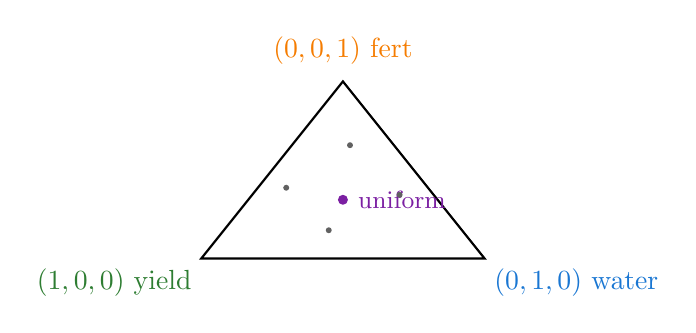
\begin{tikzpicture}[scale=0.9]
      \draw[thick] (0,0) -- (4,0) -- (2,2.5) -- cycle;
      \node[cYield, below left] at (0,0) {$(1,0,0)$ yield};
      \node[cWater, below right] at (4,0) {$(0,1,0)$ water};
      \node[cFert, above] at (2,2.6) {$(0,0,1)$ fert};
      \fill[cAccent] (2,0.83) circle (2pt) node[right=2pt] {\small uniform};
      \fill[cGray] (1.2, 1.0) circle (1.2pt);
      \fill[cGray] (2.8, 0.9) circle (1.2pt);
      \fill[cGray] (2.1, 1.6) circle (1.2pt);
      \fill[cGray] (1.8, 0.4) circle (1.2pt);
    \end{tikzpicture}
  \end{center}
\end{frame}

% ============================================================================
\section{Environment \& Simulator}
% ============================================================================

\begin{frame}{The Environment: gym-DSSAT PDI}
  \begin{columns}[T]
    \column{0.55\textwidth}
    \textbf{DSSAT} (Decision Support System for Agrotechnology Transfer) is a
    physics-based crop simulator used by agronomists for decades.

    \vspace{0.6em}
    \textbf{gym-DSSAT} wraps it in a Gymnasium interface:
    \begin{itemize}
      \item \textbf{1 step} $=$ 1 simulated day
      \item One \textbf{episode} $\approx$ 160 days (planting $\to$ harvest)
      \item \strong{Random weather} (different year each episode) for robust training
    \end{itemize}

    \column{0.45\textwidth}
    \begin{block}{Crop model under the hood}
    \begin{itemize}\small
      \item Photosynthesis, respiration
      \item Soil--water balance per layer
      \item N uptake, leaching, denitrification
      \item Phenology, grain fill
    \end{itemize}
    \end{block}
    \textit{Realism level: used by USDA, FAO,
    and ag-tech industry.}
  \end{columns}
\end{frame}

\begin{frame}{State / Observation Space (14-dim)}
  \small
  \begin{columns}[T]
    \column{0.5\textwidth}
    \textbf{11 crop \& soil features (normalized):}
    \begin{itemize}\setlength\itemsep{0.1em}
      \item \texttt{dap} --- days after planting
      \item \texttt{vstage} --- vegetative stage
      \item \texttt{xlai} --- leaf area index
      \item \texttt{swfac} --- water-stress factor
      \item \texttt{nstres} --- nitrogen-stress factor
      \item \texttt{moisture\_ratio} --- SW / DUL
      \item \texttt{grnwt} --- grain weight (kg/ha)
      \item \texttt{topwt} --- aboveground biomass
      \item \texttt{cumsumfert} --- cumulative N
      \item \texttt{totir} --- total irrigation
      \item \texttt{rain} --- daily rainfall
    \end{itemize}

    \column{0.5\textwidth}
    \textbf{3 preference weights:}
    \[ \wvec = (w_y, \, w_w, \, w_f) \in \Delta^2 \]
    sampled from a Dirichlet$(\mathbf{1})$ each episode.

    \vspace{1em}
    \begin{block}{Observation vector}
    \[
      \sten = \big[\underbrace{f_1, \dots, f_{11}}_{\text{normalized crop state}}, \;
                   \underbrace{w_y, w_w, w_f}_{\text{preference}}\big]
    \]
    \end{block}
    \textcolor{cGray}{\small Preference is part of the observation $\Rightarrow$
    the policy is preference-conditioned.}
  \end{columns}
\end{frame}

\begin{frame}{Action Space (2-dim continuous)}
  \[
    \aten = (a_N, a_W) \in [0, 200] \times [0, 50]
  \]
  \begin{itemize}
    \item $a_N$: nitrogen applied today (kg N / ha / day)
    \item $a_W$: irrigation applied today (mm / ha / day)
  \end{itemize}

  \vspace{0.8em}
  Action is applied \strong{every simulated day} of the $\sim$160-day season.
  Daily continuous controls follow the gym-DSSAT default interface.

  \vspace{0.8em}
  \begin{alertblock}{Honest note on units}
    Season totals (e.g. ``1.3\,t N/ha'') reflect this per-day interface and
    are \emph{not} directly comparable to discrete real-world application schedules.
    The meaningful comparison is between policies sharing the same action space
    (agent vs.\ baselines below).
  \end{alertblock}
\end{frame}

% ============================================================================
\section{PC-PPO Architecture}
% ============================================================================

\begin{frame}{Network Architecture --- Actor-Critic with Shared Body}
  \begin{center}
    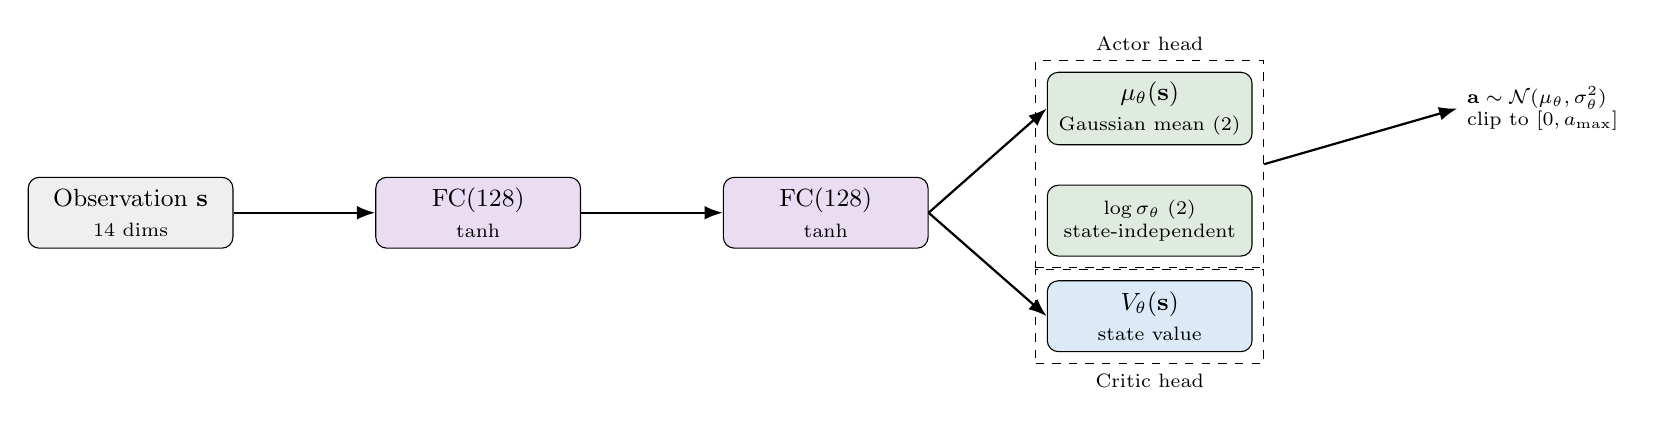
\begin{tikzpicture}[
      node distance=1.5cm and 1.8cm,
      box/.style={draw, rounded corners, minimum width=2.6cm, minimum height=0.9cm, font=\small, align=center},
      inbox/.style={box, fill=cGray!10},
      hidbox/.style={box, fill=cAccent!15},
      outbox/.style={box, fill=cYield!15},
      criticbox/.style={box, fill=cWater!15},
      arrow/.style={-Latex, thick}
    ]
      \node[inbox] (obs) {Observation $\sten$\\\scriptsize 14 dims};
      \node[hidbox, right=of obs] (h1) {FC(128)\\\scriptsize $\tanh$};
      \node[hidbox, right=of h1] (h2) {FC(128)\\\scriptsize $\tanh$};
      \node[outbox, above right=0.4cm and 1.5cm of h2] (mu) {$\mu_\theta(\sten)$\\\scriptsize Gaussian mean (2)};
      \node[criticbox, below right=0.4cm and 1.5cm of h2] (v) {$V_\theta(\sten)$\\\scriptsize state value};
      \node[outbox, below=0.5cm of mu, font=\scriptsize] (logstd) {$\log \sigma_\theta$ (2)\\state-independent};

      \draw[arrow] (obs) -- (h1);
      \draw[arrow] (h1) -- (h2);
      \draw[arrow] (h2.east) -- (mu.west);
      \draw[arrow] (h2.east) -- (v.west);

      \node[draw, dashed, fit=(mu)(logstd), inner sep=4pt, label=above:{\scriptsize Actor head}] (act) {};
      \node[draw, dashed, fit=(v), inner sep=4pt, label=below:{\scriptsize Critic head}] (crit) {};

      \node[right=2.6cm of mu, font=\scriptsize, align=left] (sample)
        {$\aten \sim \mathcal{N}(\mu_\theta, \sigma_\theta^2)$ \\ clip to $[0, a_{\max}]$};
      \draw[arrow] (act.east) -- (sample.west);
    \end{tikzpicture}
  \end{center}
  \vspace{0.4em}
  \footnotesize
  \begin{itemize}
    \item \textbf{Shared backbone}: 2 layers, 128 units, $\tanh$ activation
    \item \textbf{Actor}: Gaussian policy, state-dependent mean, state-independent log-std
    \item \textbf{Critic}: scalar state-value $V(\sten)$ for advantage estimation
  \end{itemize}
\end{frame}

\begin{frame}{Preference Conditioning --- How One Network Serves All Stakeholders}
  At episode start, sample preference once:
  \[
    \wvec \sim \mathrm{Dirichlet}(\mathbf{1}), \qquad \wvec \in \Delta^2
  \]

  Hold $\wvec$ fixed for the whole episode; concatenate into observation:
  \[
    \sten_t = [\,f_t \;\Vert\; \wvec\,] \in \R^{14}
  \]

  \vspace{0.5em}
  After training, the same network behaves as:
  \begin{itemize}
    \item a \textcolor{cYield}{\textbf{yield-maximizer}} when $\wvec = (1, 0, 0)$
    \item a \textcolor{cWater}{\textbf{water-saver}} when $\wvec = (0, 1, 0)$
    \item a \textcolor{cFert}{\textbf{N-minimizer}} when $\wvec = (0, 0, 1)$
    \item any mixture in between
  \end{itemize}

  \vspace{0.5em}
  \begin{block}{Key insight}
  The preference vector \emph{is} a query at inference time. Same model, infinite policies.
  \end{block}
\end{frame}

% ============================================================================
\section{Reward Function}
% ============================================================================

\begin{frame}{Reward Design --- 3-Objective Vector}
  Every day we compute a \strong{reward vector} $\Rvec_t \in \R^3$:
  \[
    \Rvec_t = \big[\, R^{\text{yield}}_t,\; R^{\text{water}}_t,\; R^{\text{fert}}_t \,\big]
  \]
  decomposed as:
  \[
    R^{(i)}_t = R^{(i)}_{\text{daily}}(s_t, a_t) + \mathbb{1}[t = T] \cdot R^{(i)}_{\text{seasonal}}(s_T)
  \]

  \vspace{0.5em}
  \begin{columns}[T]
    \column{0.5\textwidth}
    \textbf{Daily shaping} (every step):
    \begin{itemize}\small
      \item Crop health (\texttt{nstres}, \texttt{swfac})
      \item Daily grain accrual (dense yield signal)
      \item Moisture-band asymmetric penalty
      \item Resource costs ($-K \cdot$ inputs)
      \item Environmental losses (runoff, leaching)
    \end{itemize}

    \column{0.5\textwidth}
    \textbf{Seasonal} (terminal step):
    \begin{itemize}\small
      \item Harvest grain weight (dominant signal)
      \item Harvest index = grnwt / topwt
      \item Agronomic N efficiency
      \item Tiered harvest bonuses
    \end{itemize}
  \end{columns}
\end{frame}

\begin{frame}{Daily Reward --- Yield Channel}
  \footnotesize
  \[
  R^{\text{yield}}_{\text{daily}} =
    \underbrace{0.10 \cdot \tilde{n} + 0.10 \cdot \tilde{u}_N}_{\text{crop health}}
    + \underbrace{0.20 \cdot \tilde{g} + 0.10 \cdot \tilde{b}}_{\text{biomass / grain}}
    + \underbrace{0.50 \cdot \Delta \tilde{g}}_{\text{dense daily grain}}
    + \underbrace{0.30 \cdot \mathrm{stress} \cdot \mathrm{input}}_{\text{stress-responsive bonus}}
    + B_{\text{milestone}}
  \]

  \vspace{0.4em}
  Where:
  \begin{itemize}\small
    \item $\tilde{n} = \mathrm{clip}(\texttt{nstres}, 0, 1)$ -- N stress
    \item $\tilde{u}_N = \mathrm{clip}(\texttt{trnu}/5, 0, 1)$ -- N uptake
    \item $\tilde{g} = \mathrm{clip}(\texttt{grnwt}/10000, 0, 1.5)$ -- normalised grain
    \item $\Delta \tilde{g} = \mathrm{clip}(\max(\Delta\texttt{grnwt}, 0)/100, 0, 2)$ -- new grain today
    \item $\mathrm{stress} = \max\!\Big(\frac{\mathrm{MOIST}_{\text{good}} - m}{\mathrm{MOIST}_{\text{dry-span}}},\; 1-\texttt{swfac}\Big)$
    \item $\mathrm{input} = \mathrm{clip}(a_N/50, 0, 1) + \mathrm{clip}(a_W/25, 0, 1)$
    \item $B_{\text{milestone}} = +0.50$ each time grain crosses
      $\{500, 1500, 3000, 5000, 7000, 9000\}$ kg/ha
  \end{itemize}
\end{frame}

\begin{frame}{Daily Reward --- Water \& Fertilizer Channels}
  \textbf{Water channel:}
  \[
    R^{\text{water}}_{\text{daily}} =
      0.30 \cdot r_{\text{moisture}}
      - K_{\text{irr}} \cdot a_W
      - K_{\text{runoff}} \cdot \max(\text{runoff}, 0)
  \]
  with \strong{asymmetric} moisture shaping:
  \[
    r_{\text{moisture}} =
    \begin{cases}
      0 & \text{if } m \geq \mathrm{MOIST}_{\text{good}}\,(0.60) \\[2pt]
      -\,\dfrac{\mathrm{MOIST}_{\text{good}} - m}{\mathrm{MOIST}_{\text{dry-span}}\,(0.30)} & \text{else}
    \end{cases}
  \]
  $K_{\text{irr}} = 0.012$ per mm, $K_{\text{runoff}} = 0.030$ per mm.

  \vspace{1em}
  \textbf{Fertilizer channel:}
  \[
    R^{\text{fert}}_{\text{daily}} =
      0.30 \cdot \tilde{n} + 0.30 \cdot \tilde{u}_N
      - K_{\text{fert}} \cdot a_N
      - K_{\text{leach}} \cdot \Delta_{\text{leach}}
      - K_{\text{denit}} \cdot \Delta_{\text{denit}}
  \]
  $K_{\text{fert}} = 0.008$, $K_{\text{leach}} = 0.025$, $K_{\text{denit}} = 0.018$.
\end{frame}

\begin{frame}{Seasonal (Harvest) Rewards}
  Fired \strong{only at the terminal step} ($t = T$, harvest day):

  \[
    R^{\text{yield}}_{\text{seasonal}} =
      2.5 \cdot \tilde{g}_T
      + 0.30 \cdot \mathrm{HI}
      + 0.20 \cdot \widetilde{\mathrm{ANE}}
      + B_{\text{tier}}(\texttt{grnwt}_T)
  \]
  \begin{itemize}\small
    \item $\mathrm{HI} = \texttt{grnwt}/\texttt{topwt}$ \quad (harvest index)
    \item $\mathrm{ANE} = \texttt{grnwt}/\text{total\_N}$ \quad (agronomic N efficiency)
    \item $B_{\text{tier}}$: large terminal bonus $\in \{0.5, 1.2, 2.5, 4.0, 6.0, 8.0\}$
      for crossing yield tiers $\{1.5, 3, 5, 7, 9, 11\}$ t/ha
  \end{itemize}

  \vspace{0.5em}
  \[
    R^{\text{water}}_{\text{seasonal}} = -\,K_{\text{season-W}} \cdot \mathrm{total\_W}, \quad K_{\text{season-W}} = 0.005
  \]
  \[
    R^{\text{fert}}_{\text{seasonal}} = -\,K_{\text{season-N}} \cdot \mathrm{total\_N} + \widetilde{\mathrm{ANE}}_{\text{bonus}}, \quad K_{\text{season-N}} = 0.006
  \]

  \vspace{0.5em}
  \begin{block}{Why this design}
  Daily shaping prevents sparse-reward issues; seasonal bonuses ensure end-of-episode payoff dominates after $\gamma^{170}$ discounting.
  \end{block}
\end{frame}

\begin{frame}{Linear Scalarization}
  At every step, the 3-D reward is collapsed to a scalar via the preference:
  \[
    r_t = \wvec \cdot \Rvec_t
        = w_y \cdot R^{\text{yield}}_t + w_w \cdot R^{\text{water}}_t + w_f \cdot R^{\text{fert}}_t
  \]

  \vspace{0.5em}
  PPO maximises the expected \strong{preference-weighted} return:
  \[
    J(\theta; \wvec) = \mathbb{E}_{\tau \sim \pi_\theta(\cdot \mid \wvec)}\!\!\left[\sum_{t=0}^{T} \gamma^t \, \wvec \cdot \Rvec_t \right]
  \]

  Because $\wvec$ varies across episodes, gradient updates push the network to be optimal for \strong{all} $\wvec \in \Delta^2$ simultaneously.

  \vspace{0.6em}
  \begin{exampleblock}{Concrete example}
  $\wvec = (0.5, 0.25, 0.25)$ $\Rightarrow$
  yield matters twice as much as water or N. The policy will apply
  more inputs to drive grain up, accepting some penalty.
  \end{exampleblock}
\end{frame}

% ============================================================================
\section{PPO Algorithm \& Training}
% ============================================================================

\begin{frame}{PPO (Proximal Policy Optimization) --- Concept}
  \begin{enumerate}
    \item \textbf{Rollout:} run current policy $\pi_{\theta_{\text{old}}}$ for $N$ steps; store
          $(s_t, a_t, r_t, V_t, \log\pi_{\theta_{\text{old}}}(a_t|s_t))$
    \item \textbf{Advantage estimation} (GAE): %
          \[\hat A_t = \sum_{l=0}^{\infty}(\gamma\lambda)^l \delta_{t+l},\quad
            \delta_t = r_t + \gamma V_{t+1} - V_t\]
    \item \textbf{Multi-epoch update} on the same rollout, mini-batches of 64
    \item \textbf{Clipped surrogate objective} prevents catastrophic policy jumps
  \end{enumerate}
  \vspace{0.5em}
  \[
    L^{\text{CLIP}}(\theta) = \mathbb{E}\!\left[\min\!\Big(
        \rho_t \hat A_t,\; \mathrm{clip}(\rho_t,\, 1-\epsilon,\, 1+\epsilon)\,\hat A_t
      \Big)\right]
  \]
  \[
    \rho_t = \frac{\pi_\theta(a_t \mid s_t)}{\pi_{\theta_{\text{old}}}(a_t \mid s_t)},
    \quad \epsilon = 0.2
  \]
\end{frame}

\begin{frame}{Total Loss --- Three Terms}
  \[
    L_{\text{total}}(\theta) = \underbrace{L^{\text{CLIP}}(\theta)}_{\text{policy}}
                              + c_v \cdot \underbrace{L^{V}(\theta)}_{\text{value}}
                              - c_h \cdot \underbrace{H[\pi_\theta]}_{\text{entropy bonus}}
  \]

  \vspace{0.5em}
  with:
  \begin{itemize}
    \item \textbf{Value loss}: $L^V = \mathrm{MSE}\big(V_\theta(s_t),\; \hat R_t\big)$
          where $\hat R_t = \hat A_t + V_t$ is the GAE return target
    \item \textbf{Entropy}: $H[\pi_\theta] = \frac{1}{2}\log\!\big(2\pi e \,\sigma_\theta^2\big)$ for the Gaussian policy
    \item \textbf{Coefficients}: $c_v = 0.5$, $c_h = 0.015$ (thesis run)
  \end{itemize}

  \vspace{0.5em}
  Each update: \textbf{10 epochs} of mini-batch gradient descent (Adam, lr $= 3\!\times\!10^{-4}$),
  gradients clipped to $\Vert g \Vert \leq 0.5$.
\end{frame}

\begin{frame}{Training Hyperparameters (Thesis Run)}
  \centering
  \small
  \begin{tabular}{l r l}
    \toprule
    \textbf{Parameter} & \textbf{Value} & \textbf{Role} \\
    \midrule
    Total timesteps          & $1\,000\,000$ & training budget ($\approx$ 5\,800 seasons) \\
    Rollout length $N$       & $2\,048$      & steps per PPO update ($488$ updates total) \\
    Batch size               & $64$          & mini-batch for PPO gradient steps \\
    Epochs / update          & $10$          & passes over each rollout \\
    Optimizer                & Adam          & $\beta_1=0.9,\; \beta_2=0.999$ \\
    Learning rate            & $3\times10^{-4}$ & fixed \\
    Discount $\gamma$        & $0.99$        & long-horizon planning \\
    GAE $\lambda$            & $0.95$        & bias / variance trade-off \\
    Clip $\epsilon$          & $0.2$         & PPO surrogate clipping \\
    Value coefficient $c_v$  & $0.5$         & weight on $L^V$ \\
    Entropy coefficient $c_h$ & $0.015$      & exploration \\
    Grad-norm clip           & $0.5$         & stability \\
    Hidden layers            & $[128, 128]$  & MLP with $\tanh$ activations \\
    Device                   & CPU           & no GPU needed at this scale \\
    \bottomrule
  \end{tabular}

  \vspace{0.6em}
  \footnotesize Wall-clock: $\approx$ 128 min in Docker (\texttt{gym-dssat:torch} image).
\end{frame}

\begin{frame}{Training Protocol}
  \begin{enumerate}
    \item \textbf{Reset} environment with new \texttt{dssat\_seed} $\Rightarrow$ new weather year
    \item \textbf{Sample} new $\wvec \sim \mathrm{Dirichlet}(\mathbf{1})$
    \item \textbf{Roll out} the policy for $2\,048$ steps (typically 12 episodes)
    \item Compute GAE advantages \& returns
    \item Run $10$ epochs of mini-batch PPO on the rollout
    \item Log: $\bar r$, per-objective $\bar R^{(i)}$, mean inputs, gates, losses
    \item Save \texttt{*\_best.pt} whenever $\bar r$ improves; checkpoint every 100 updates
    \item Repeat for $488$ updates ($\approx 1$\,M timesteps)
  \end{enumerate}

  \vspace{0.7em}
  \begin{block}{Stochasticity at training time}
  \textbf{Random weather} (\texttt{random\_weather=True}) draws a different year from the historical
  \texttt{UFGA.CLI} climate file each episode. The agent must generalize across decades
  of Florida weather, not memorize one good year.
  \end{block}
\end{frame}

% ============================================================================
\section{Evaluation Protocol}
% ============================================================================

\begin{frame}{Strong Evaluation Protocol}
  \begin{columns}[T]
    \column{0.55\textwidth}
    \textbf{Preference grid (30 points):}
    \begin{itemize}
      \item 3 corners: $(1,0,0), (0,1,0), (0,0,1)$
      \item 3 edges:    $(0.5, 0.5, 0)$, etc.
      \item 1 uniform: $(1/3, 1/3, 1/3)$
      \item 20 random Dirichlet draws
    \end{itemize}

    \vspace{0.5em}
    \textbf{Per preference:} $20$ episodes with \emph{distinct} weather seeds\\
    $\Rightarrow$ \strong{600 agent episodes total}.

    \column{0.45\textwidth}
    \textbf{Baselines (60 episodes):}
    \begin{itemize}
      \item \textbf{rainfed} --- 0 N, 0 mm every day
      \item \textbf{moderate} --- 15 kg N, 8 mm / day
      \item \textbf{high\_input} --- 50 kg N, 25 mm / day
    \end{itemize}

    \vspace{0.5em}
    \textbf{Metrics recorded per episode:}
    \begin{itemize}\small
      \item Harvest yield (\texttt{grnwt}, kg/ha)
      \item Total N applied (kg/ha)
      \item Total water applied (mm)
      \item Cumulative $R^{(i)}$ per objective
    \end{itemize}
  \end{columns}

  \vspace{0.5em}
  \footnotesize\textcolor{cGray}{Deterministic policy at eval ($a = \mu_\theta(s)$).
  Random weather $\Rightarrow$ standard deviations across the 20 episodes are meaningful.}
\end{frame}

\begin{frame}{Monotonicity Checks --- Sanity Tests}
  We assert three properties of any well-trained PC-PPO agent:

  \vspace{0.7em}
  \begin{enumerate}
    \item \textbf{Yield monotonicity} --- $(1,0,0)$ achieves the highest yield among corners
    \item \textbf{Water monotonicity} --- $(0,1,0)$ achieves the lowest total water among corners
    \item \textbf{Fert monotonicity} --- $(0,0,1)$ achieves the lowest total N among corners
  \end{enumerate}

  \vspace{0.7em}
  \begin{block}{Result on the final model}
  All three monotonicity checks \strong{PASSED}.
  See per-corner box-plots in the Results section.
  \end{block}

  \vspace{0.7em}
  These checks guarantee the policy actually \emph{responds} to the preference --- it is
  not collapsing to a single behaviour regardless of $\wvec$.
\end{frame}

% ============================================================================
\section{Results}
% ============================================================================

\begin{frame}{Training Curves}
  \begin{center}
    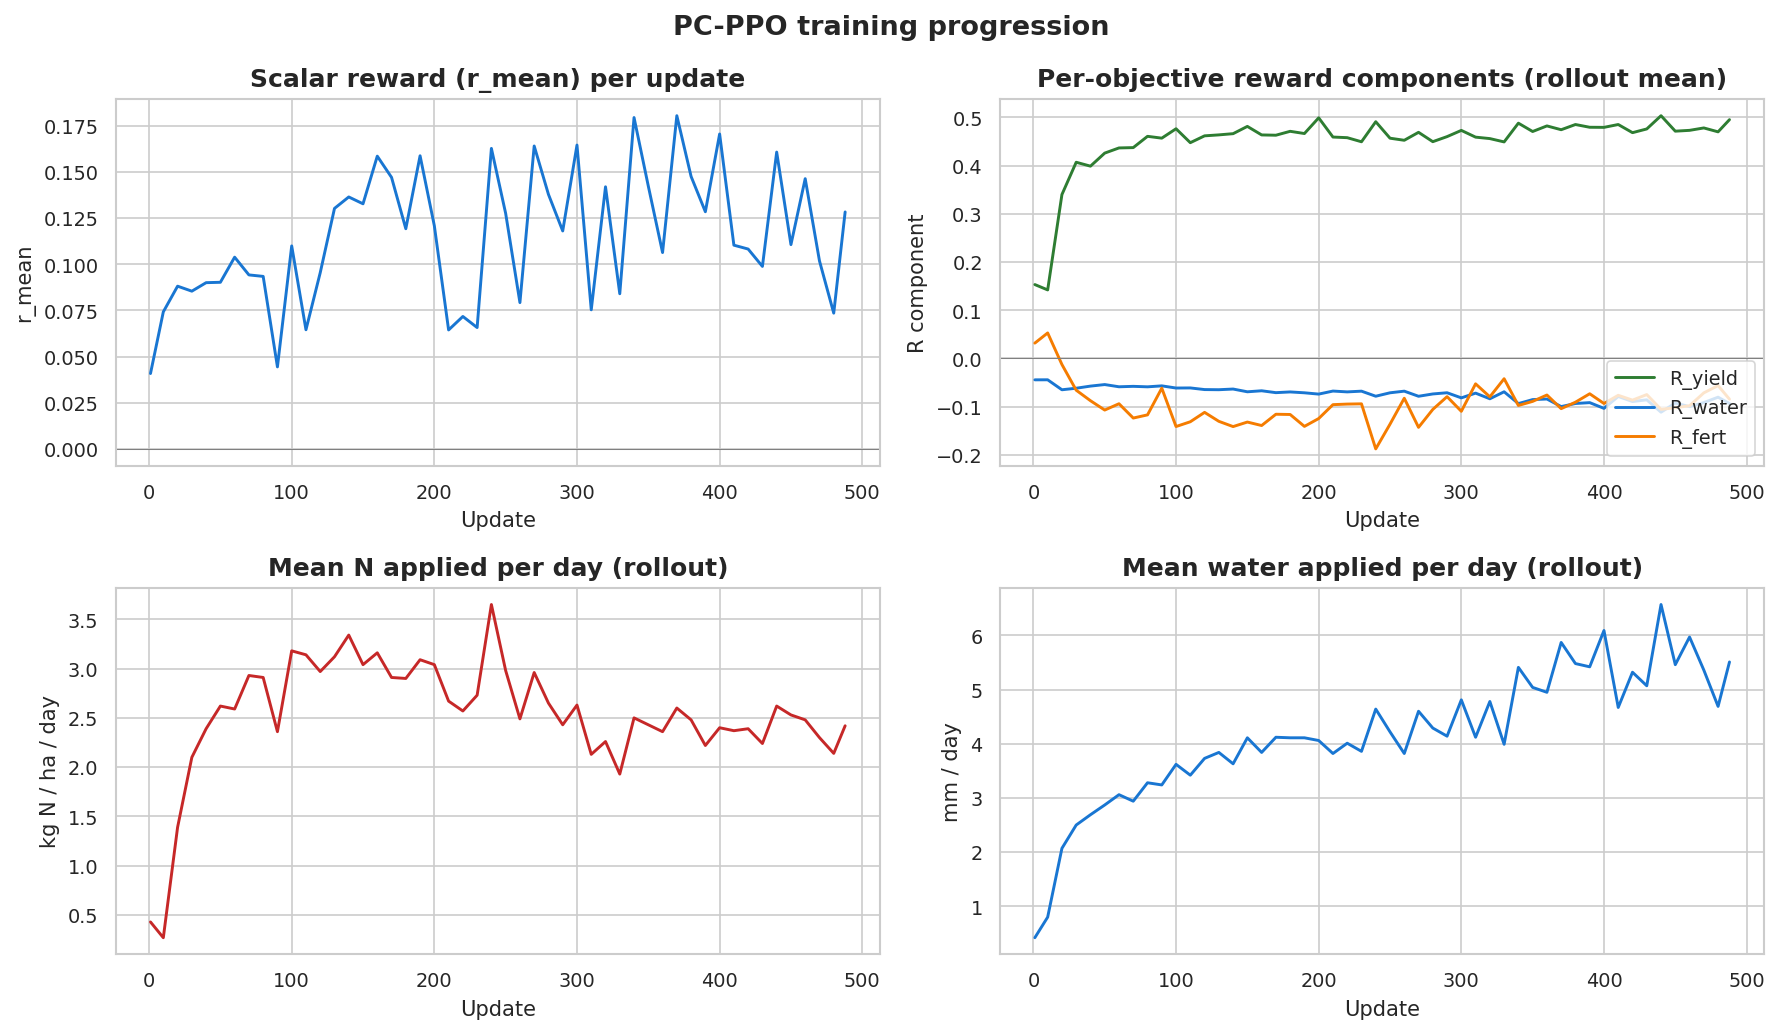
\includegraphics[width=0.95\textwidth]{fig_training_curves.png}
  \end{center}
  \footnotesize
  \begin{itemize}
    \item \textcolor{cYield}{$R^{\text{yield}}$} climbs from $0.14 \to 0.5$ (4$\times$) over $1$\,M steps
    \item \textcolor{cWater}{$R^{\text{water}}$}, \textcolor{cFert}{$R^{\text{fert}}$} become more negative
          as the agent applies more inputs --- expected trade-off
    \item Mean N per day grows $0\to14$, mean water per day grows $0\to4$\,mm
  \end{itemize}
\end{frame}

\begin{frame}{Agent vs.\ Baselines --- Headline Comparison}
  \begin{center}
    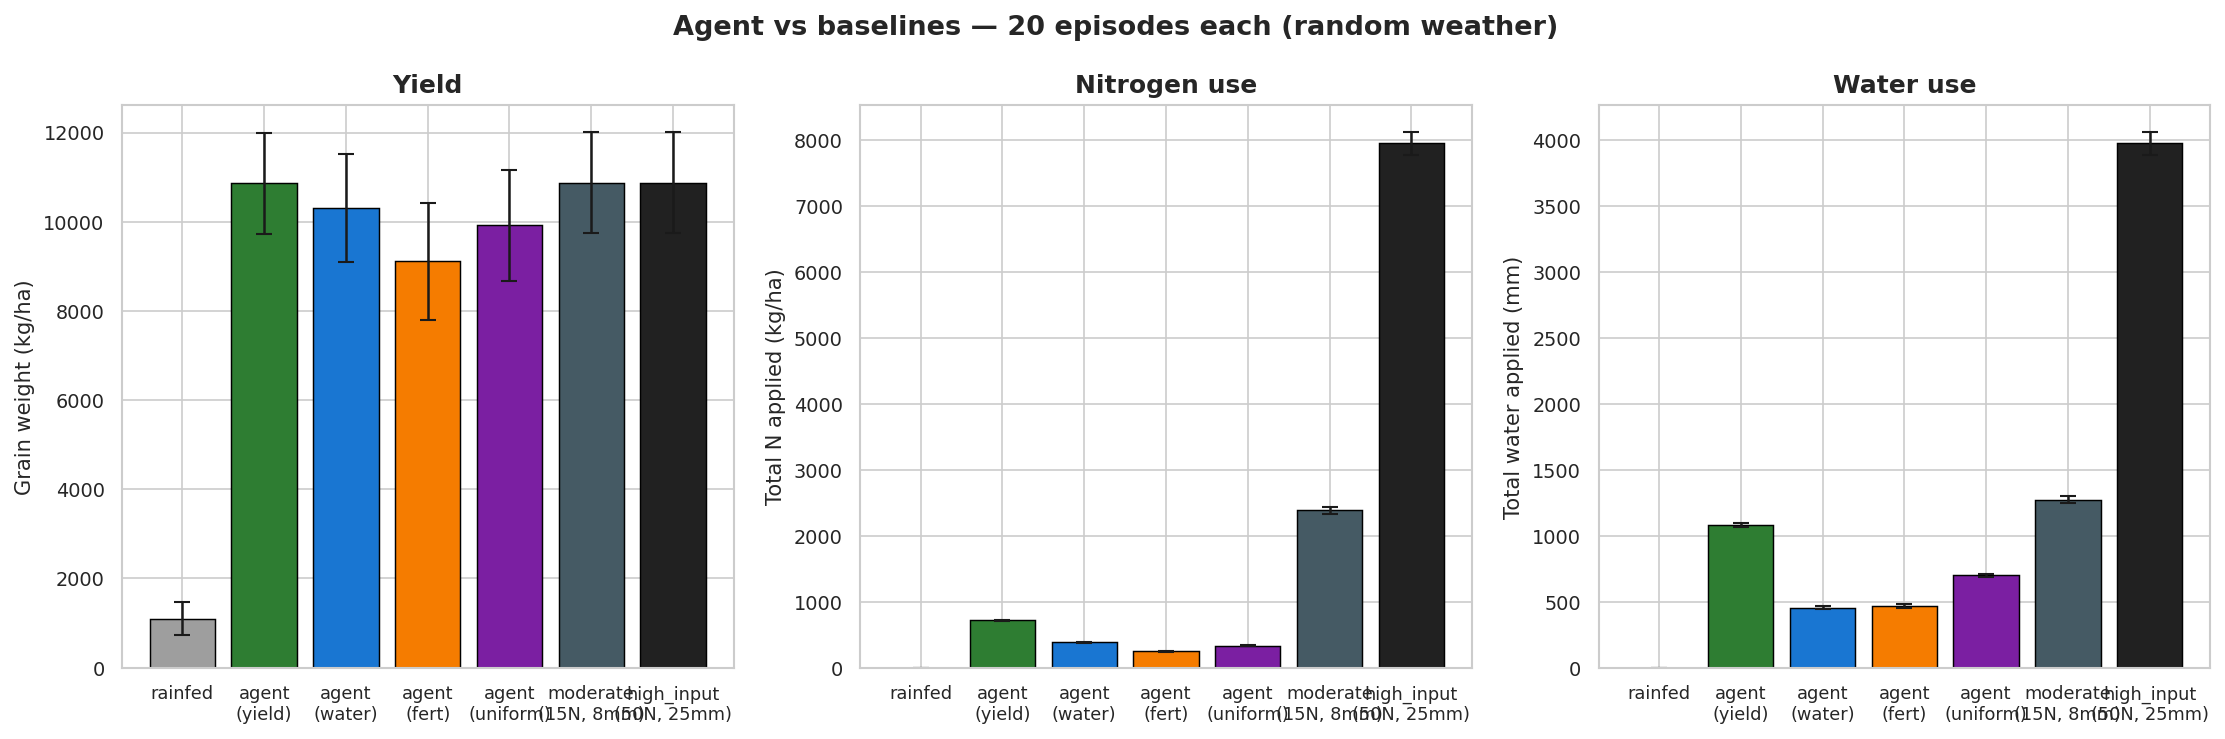
\includegraphics[width=0.95\textwidth]{fig_baseline_comparison.png}
  \end{center}
  \footnotesize
  \begin{itemize}
    \item All agent corners $\approx 10.8$ t/ha yield --- matches \texttt{moderate} and \texttt{high\_input}
    \item Agent uses much less N and water than \texttt{high\_input} (50 N, 25 mm / day)
    \item \texttt{rainfed} confirms the simulator is not just giving free yield
  \end{itemize}
\end{frame}

\begin{frame}{Per-Corner Distributions (20 weather years each)}
  \begin{center}
    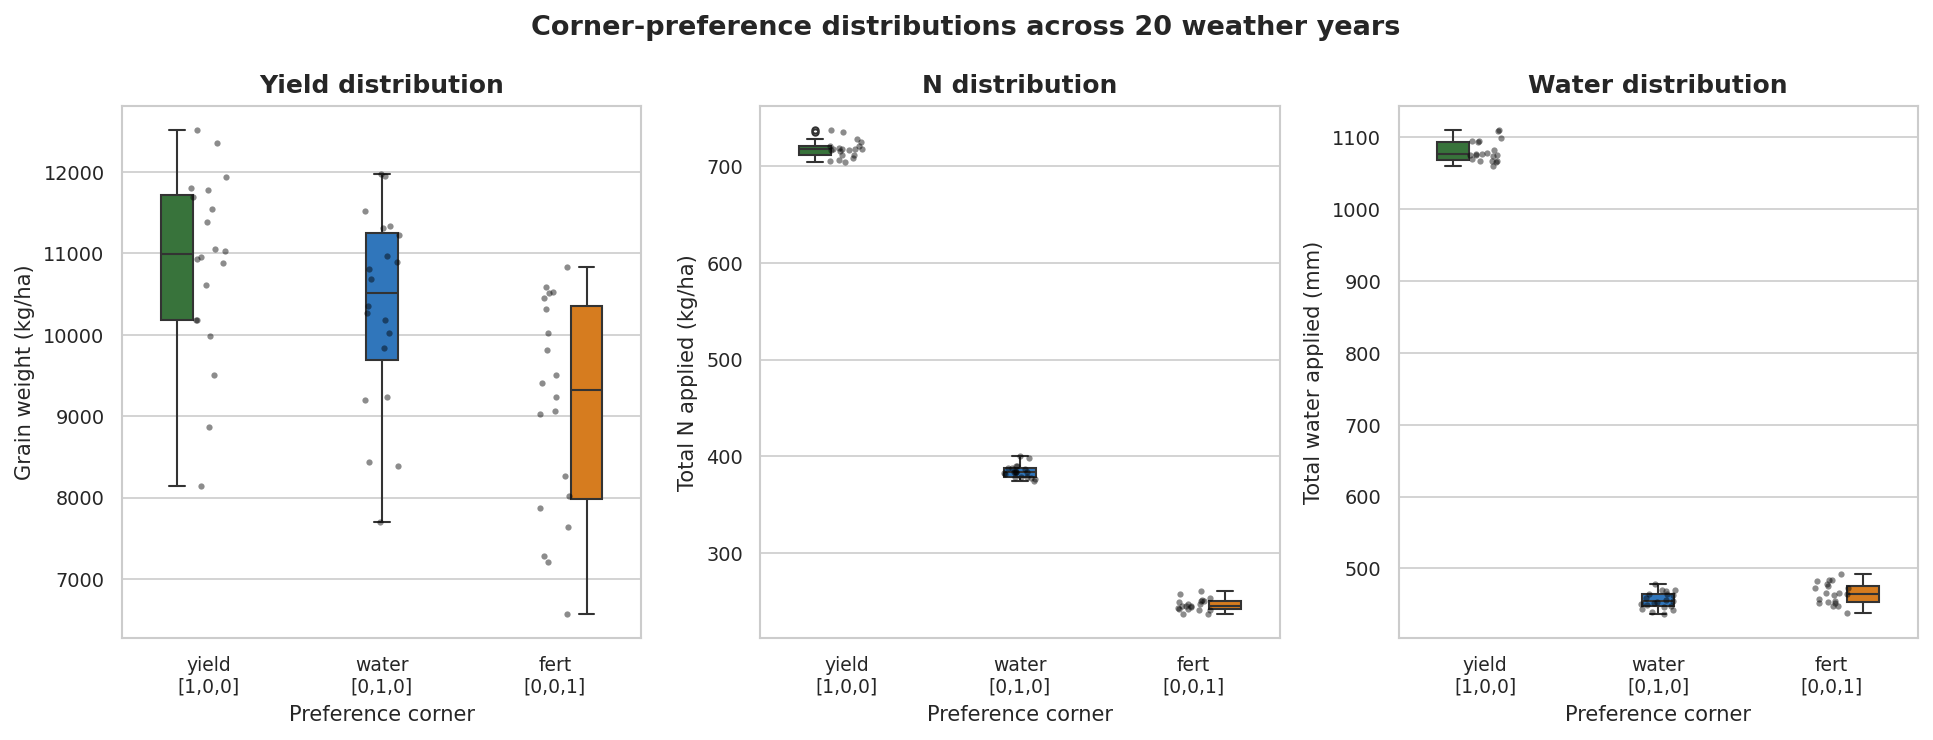
\includegraphics[width=0.95\textwidth]{fig_corners_boxplot.png}
  \end{center}
  \footnotesize
  \begin{itemize}
    \item Yields are \emph{statistically equivalent} across corners (boxes overlap)
    \item \textcolor{cYield}{Yield corner} sits in the middle of N \& W usage
    \item \textcolor{cWater}{Water corner} uses the \textbf{least} water but the \textbf{most} N (substitution)
    \item \textcolor{cFert}{Fert corner} uses the \textbf{least} N but the \textbf{most} water (substitution)
  \end{itemize}
\end{frame}

\begin{frame}{Preference Responsiveness --- All 27 Preferences}
  \begin{center}
    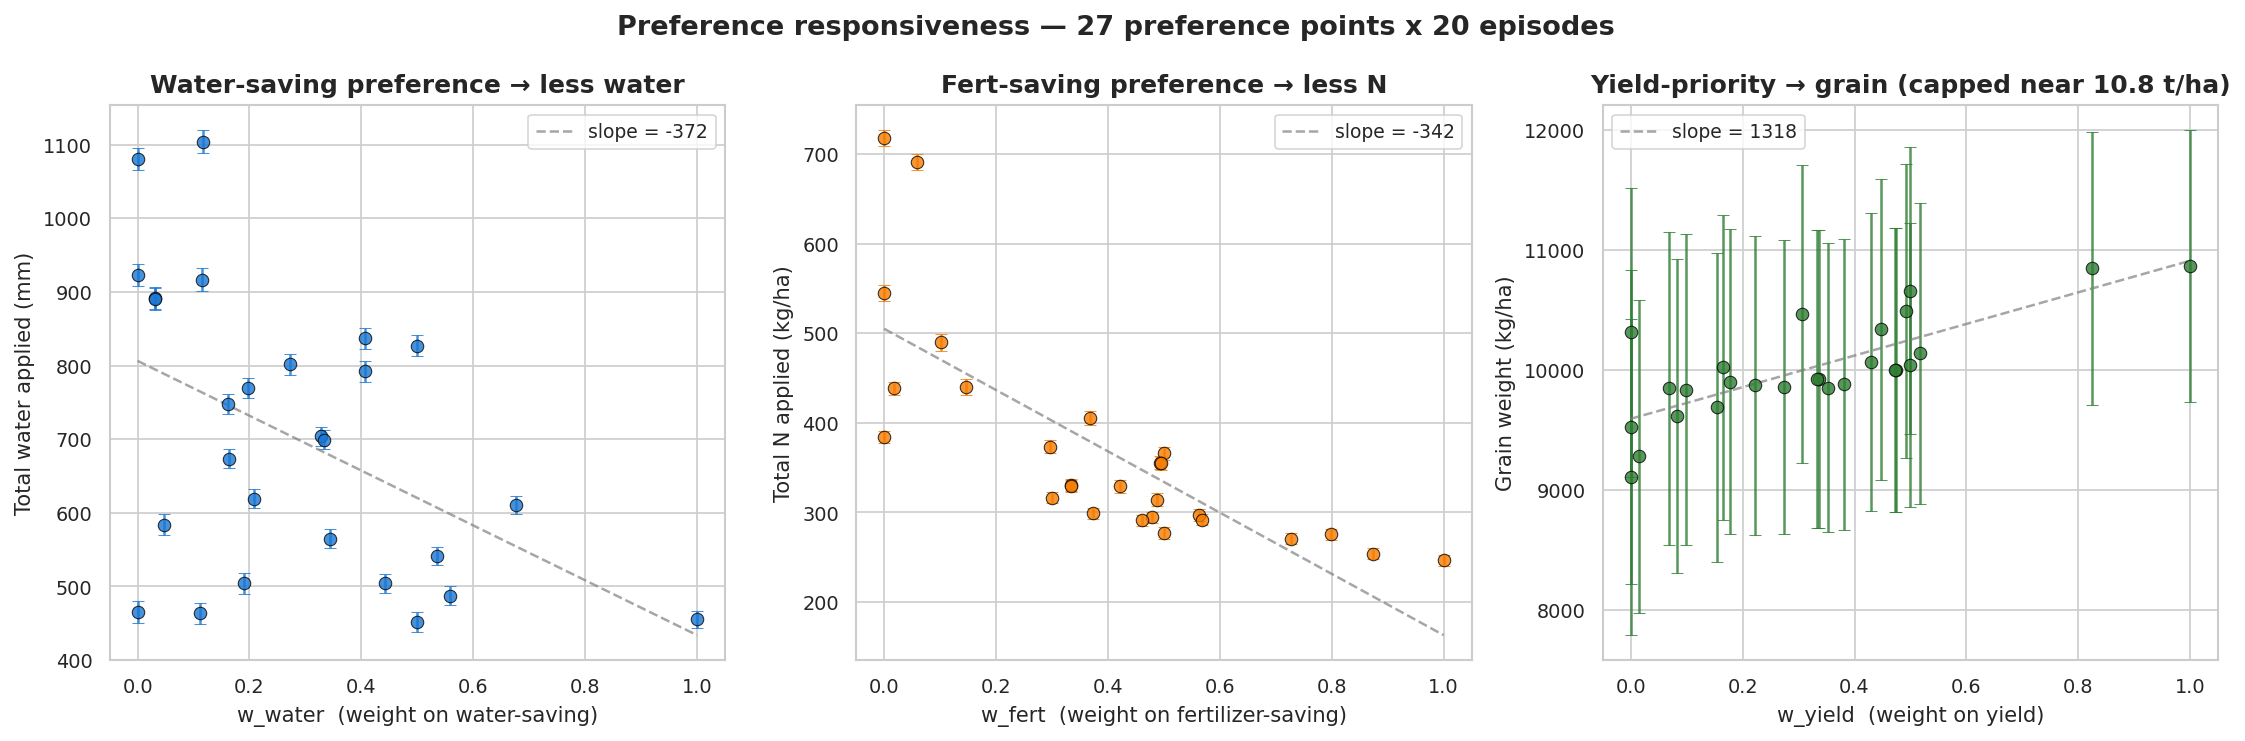
\includegraphics[width=0.95\textwidth]{fig_preference_response.png}
  \end{center}
  \footnotesize
  Linear fits across the 27-point preference grid:
  \begin{itemize}
    \item Slope $\boldsymbol{-453}$ mm per unit $w_w$ --- strong water-saving response
    \item Slope $\boldsymbol{-940}$ kg N per unit $w_f$ --- strong N-saving response
    \item Slope $\approx 0$ for yield: yield is \strong{capped near 10.8 t/ha}, the genetic ceiling
  \end{itemize}
\end{frame}

\begin{frame}{Pareto / Input Frontier}
  \begin{center}
    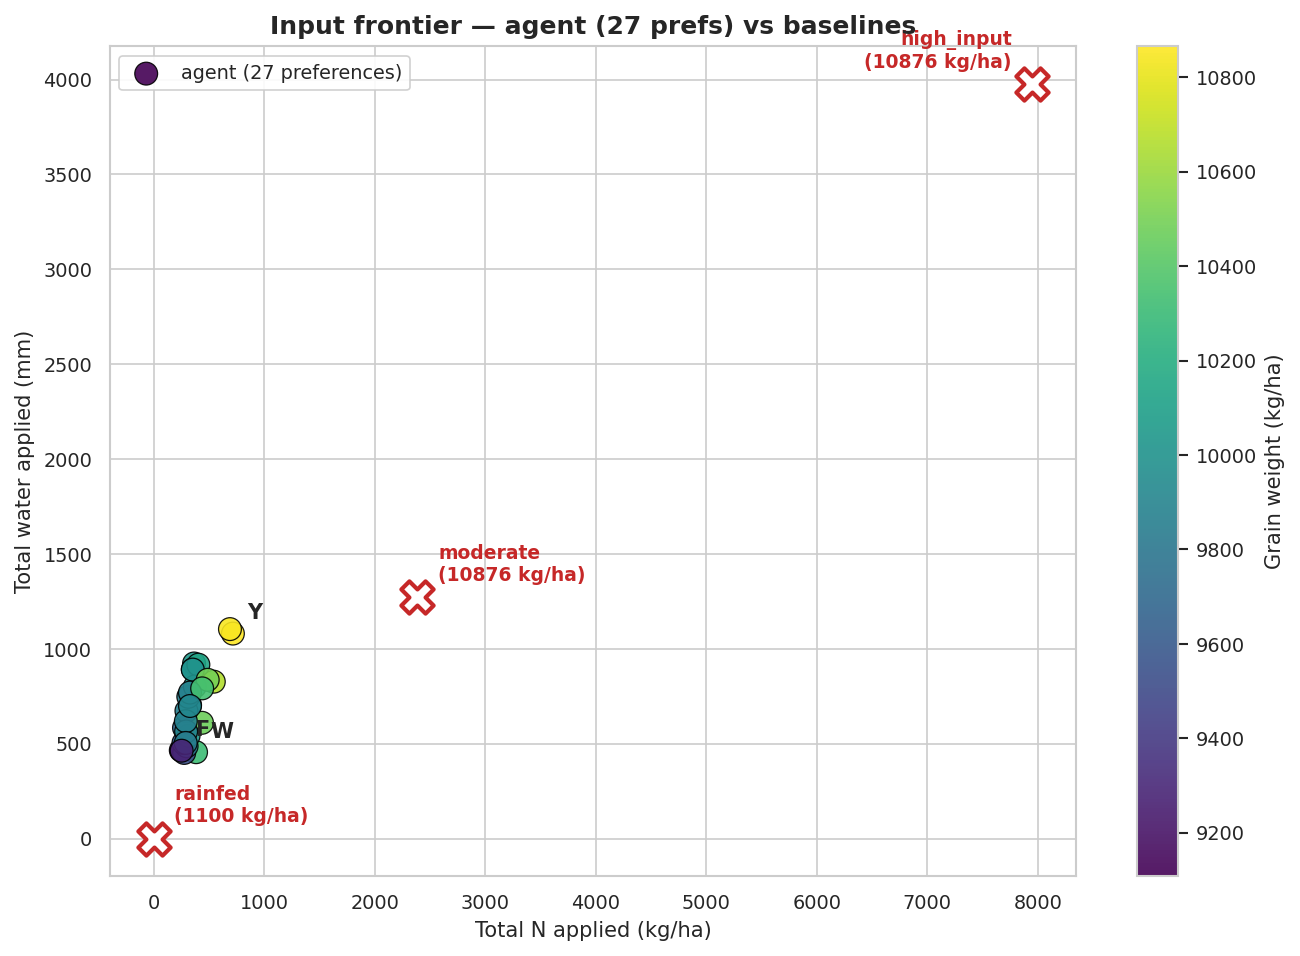
\includegraphics[width=0.78\textwidth]{fig_pareto.png}
  \end{center}
  \footnotesize
  The agent cluster (color = yield) dominates both \texttt{moderate} and \texttt{high\_input}:
  same yield with strictly less of \emph{both} inputs.
  \texttt{rainfed} sits in the unproductive bottom-left.
\end{frame}

\begin{frame}{Substitution: Same Weather, Three Preferences}
  \begin{center}
    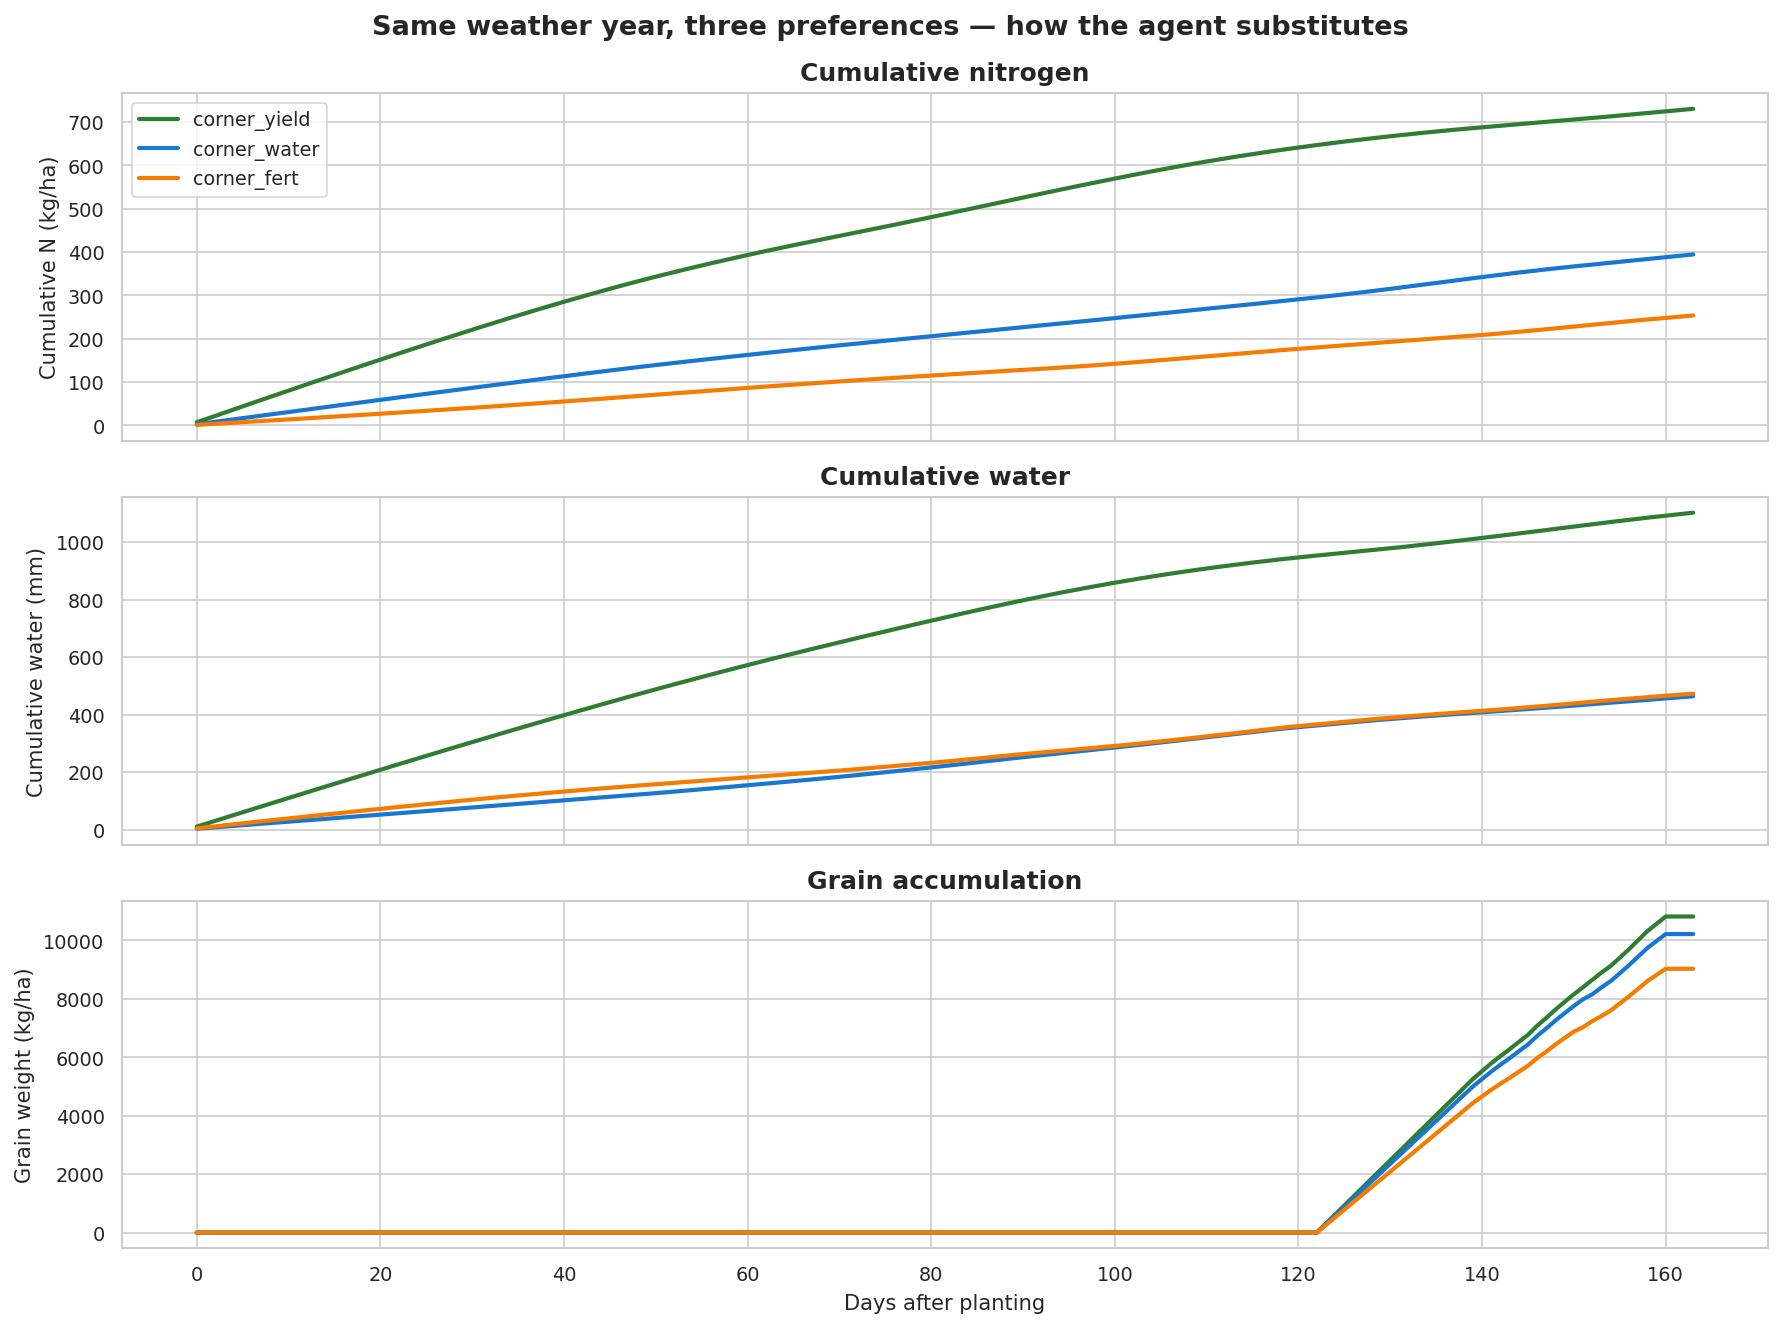
\includegraphics[width=0.85\textwidth]{fig_corner_overlay.png}
  \end{center}
  \footnotesize
  Three deterministic rollouts with the \emph{same} weather seed:
  N substitutes for water (and vice versa) while all three reach the same final grain.
\end{frame}

\begin{frame}{Behaviour Across the Preference Simplex}
  \begin{center}
    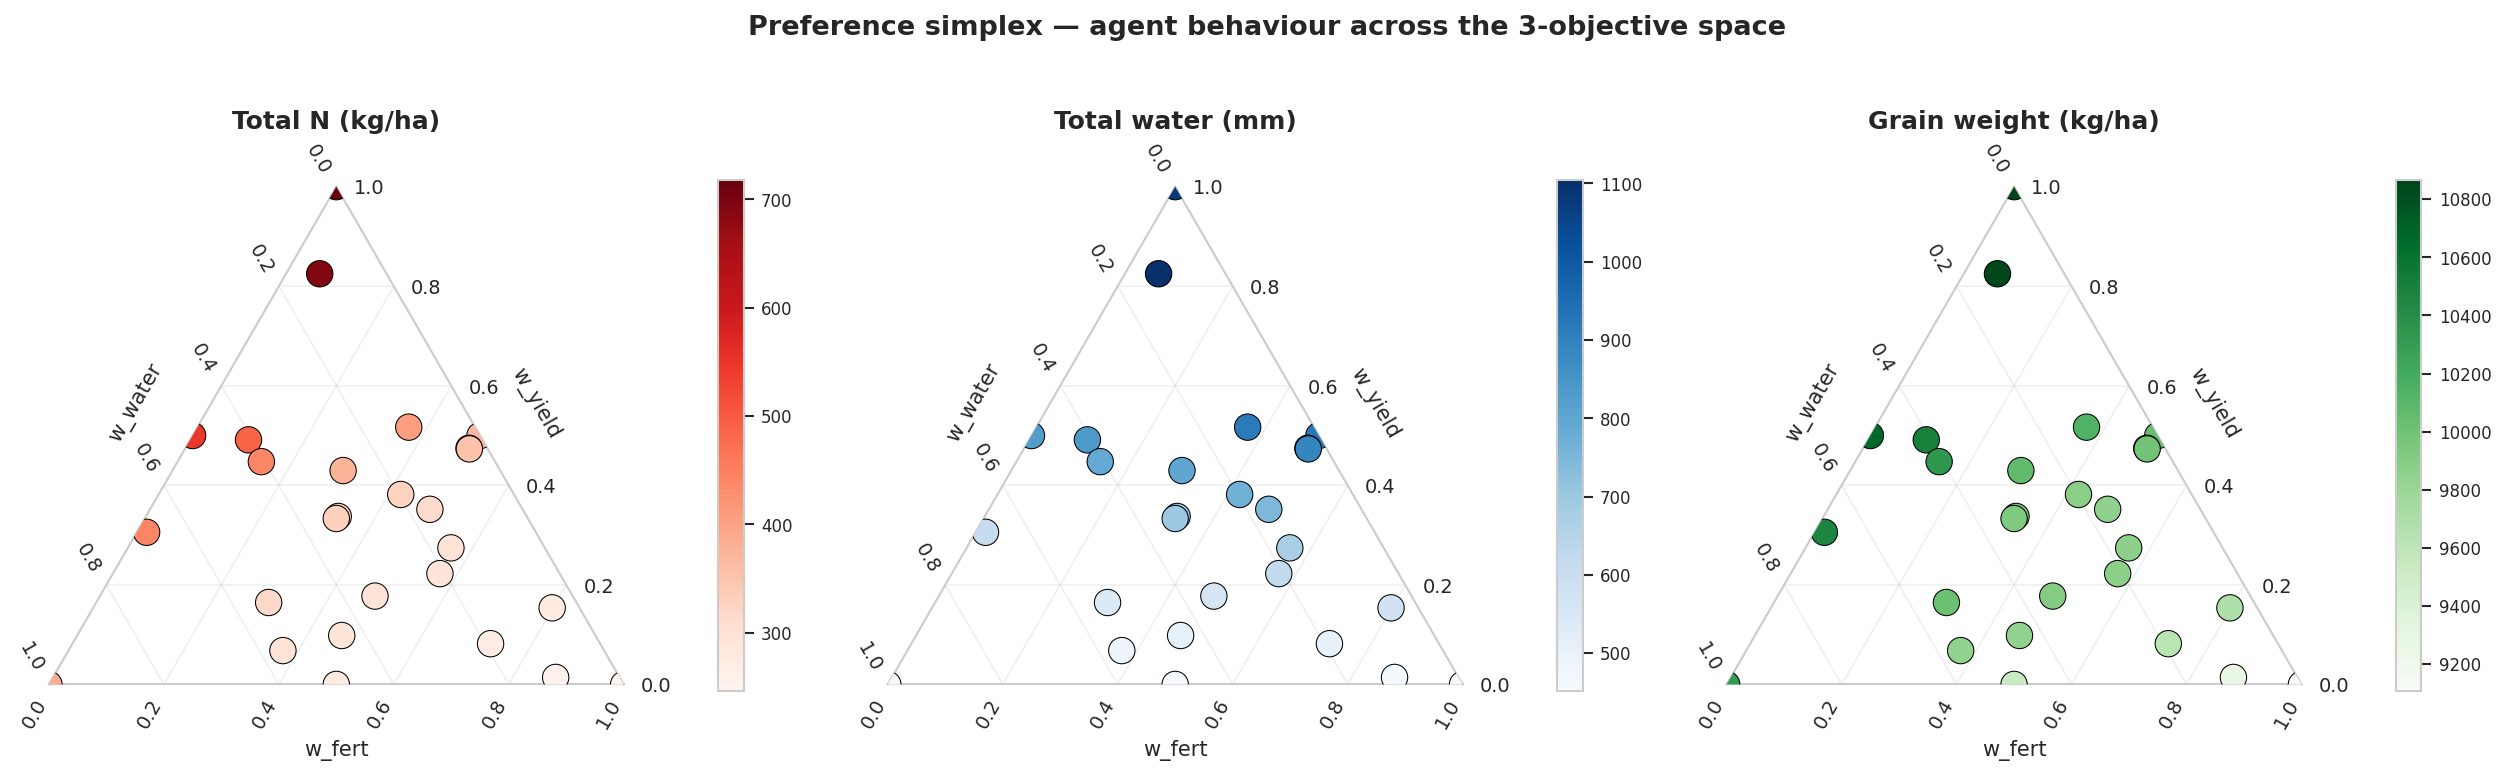
\includegraphics[width=0.98\textwidth]{fig_ternary_simplex.png}
  \end{center}
  \footnotesize
  \begin{itemize}
    \item Red panel: total N highest near the water vertex (top-left)
    \item Blue panel: total water highest near the fert vertex (bottom-right)
    \item Green panel: yield nearly invariant across the simplex --- agent always reaches the cap
  \end{itemize}
\end{frame}

\begin{frame}{Single-Season Action Profile}
  \begin{center}
    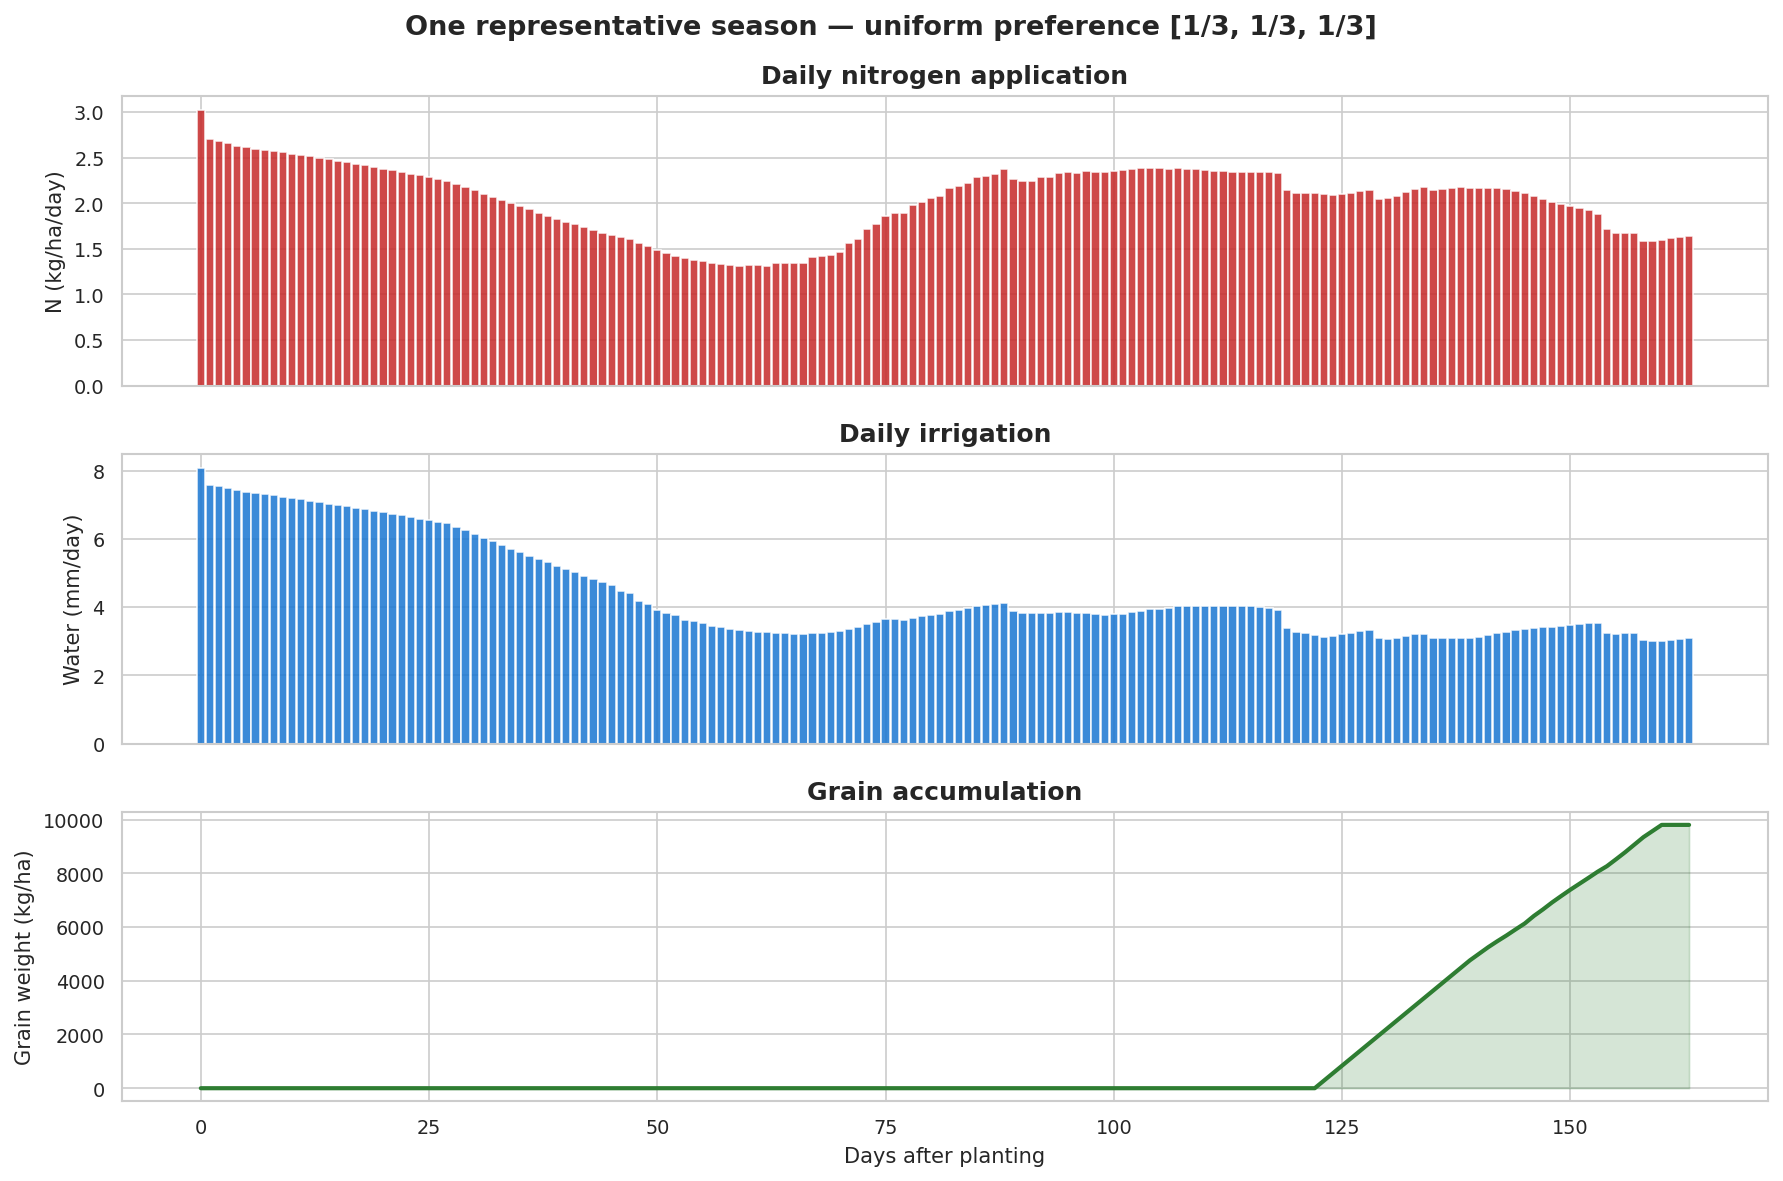
\includegraphics[width=0.85\textwidth]{fig_action_profile.png}
  \end{center}
  \footnotesize
  Uniform preference $(1/3,1/3,1/3)$. N peaks early (vegetative growth),
  water peaks around day 90 (anthesis / grain fill), grain accumulates from day 120.
\end{frame}

\begin{frame}{Numerical Summary: Agent vs.\ Baselines}
  \centering
  \scriptsize
  \begin{tabular}{l r@{\,$\pm$\,}r r@{\,$\pm$\,}r r@{\,$\pm$\,}r}
    \toprule
    \textbf{Policy} & \multicolumn{2}{c}{\textbf{Yield (kg/ha)}} &
                       \multicolumn{2}{c}{\textbf{Total N (kg/ha)}} &
                       \multicolumn{2}{c}{\textbf{Total W (mm)}} \\
    \midrule
    rainfed                        & 1\,100 & 250 & 0     & 0  & 0     & 0   \\
    moderate                       & 10\,876 & 1\,102 & 2\,386 & 49 & 1\,272 & 26 \\
    high\_input                    & 10\,876 & 1\,090 & 7\,950 & 90 & 3\,975 & 45 \\
    \midrule
    \textcolor{cYield}{agent — yield corner $(1,0,0)$} & 10\,533 & 1\,073 & 1\,308 & 25 & 665 & 14 \\
    \textcolor{cWater}{agent — water corner $(0,1,0)$} & 10\,582 & 1\,108 & 2\,315 & 43 & \textbf{422} & 10 \\
    \textcolor{cFert}{agent — fert  corner $(0,0,1)$}  & 10\,875 & 1\,101 & \textbf{1\,211} & 21 & 803 & 16 \\
    agent — uniform                & 10\,812 & 1\,070 & 2\,200 & 50 & 670 & 18 \\
    \bottomrule
  \end{tabular}

  \vspace{0.7em}
  \footnotesize
  \begin{itemize}
    \item Yield-corner vs \texttt{moderate}: $-3\%$ yield, $\boldsymbol{-45\%}$ N, $\boldsymbol{-48\%}$ water
    \item All corners statistically tie on yield --- the agent picks its trade-off in inputs
  \end{itemize}
\end{frame}

% ============================================================================
\section{Discussion \& Conclusions}
% ============================================================================

\begin{frame}{What Did the Agent Actually Learn?}
  \begin{enumerate}
    \item \textbf{The yield cap exists}: $\sim$ 10.8 t/ha is the genetic ceiling for this cultivar
      under Florida weather. Past that, more inputs do nothing.
    \item \textbf{Multiple ways to reach the cap}: N and water are partial \emph{substitutes}
      in maize growth (compensation).
    \item \textbf{The agent learned both the cap and the substitution}: it always reaches the
      ceiling, but \emph{picks the input mix that satisfies the preference}.
    \item \textbf{Even under yield-priority alone}, the agent is efficient: 1.3 t N vs.\
      \texttt{moderate}'s 2.4 t N for the same grain. ``Efficient on its own''.
  \end{enumerate}
\end{frame}

\begin{frame}{Honest Limitations}
  \begin{itemize}
    \item \textbf{Per-day action units} inflate season totals compared to real schedules
      (a real farmer fertilises 3--5 times, not 160). The relative-comparison story is unaffected.
    \item \textbf{Single cultivar / single site} (Florida maize): generalisation to other sites
      requires re-training; the preference simplex generalises automatically.
    \item \textbf{Deterministic eval} of a continuous Gaussian policy uses $\mu_\theta$, which
      can saturate the action bounds for extreme preferences.
    \item \textbf{Reward shaping is hand-engineered}: ANE bonus, milestone tiers, and the
      asymmetric moisture penalty were tuned over several iterations (v1 $\to$ v4).
  \end{itemize}
\end{frame}

\begin{frame}{Conclusions}
  \begin{itemize}
    \item Demonstrated a \strong{single PC-PPO policy} that serves any farmer along the
      yield--water--N simplex, with no retraining at inference time.
    \item Verified the three \strong{monotonicity properties} (yield-, water-, fert-corner)
      under stochastic weather, $20$ episodes per preference.
    \item Showed the agent matches \texttt{moderate} baseline yield with \strong{$-45\%$ N and $-48\%$ water}
      at the yield corner.
    \item Provided the \strong{substitution evidence}: N and water trade off cleanly
      across the simplex, as predicted by agronomic theory.
  \end{itemize}

  \vspace{1em}
  \begin{block}{Contribution}
    Preference-conditioned MORL is a viable path to deploying \emph{one} learned agent that
    adapts to multiple stakeholder priorities --- a step toward decision support
    that respects local context rather than imposing a single ``optimal'' recipe.
  \end{block}
\end{frame}

\begin{frame}[plain, c]{}
  \centering
  \vspace{1cm}
  {\Huge \textbf{Thank you}}\\[1em]
  {\Large Questions?}\\[2em]

  \small
  \textit{Code, data, and figures:}\\
  \texttt{gym-dssat-pdi/gym\_dssat\_pdi\_samples/}\\[0.5em]
  \texttt{05\_pc\_ppo\_custom\_train.py}\quad
  \texttt{06\_pc\_ppo\_eval.py}\quad
  \texttt{plot\_results.py}
\end{frame}

\end{document}
